\documentclass[journal,a4paper]{IEEEtran}

% IEEE-style report;
\usepackage[T1]{fontenc}
\usepackage{amsmath,amsfonts,amssymb,amsthm}
\usepackage{graphicx}
\usepackage{url}
\usepackage[numbers,sort&compress]{natbib}
\usepackage{hyperref}
\usepackage{booktabs}
\usepackage{tabularx}
\usepackage{array}
\usepackage{tikz}
\usetikzlibrary{arrows.meta,positioning,calc}
\usepackage{enumitem}
\usepackage{microtype}
\usepackage{comment}
\usepackage{float}

\hypersetup{colorlinks=true, linkcolor=black, urlcolor=blue, citecolor=black}
\setlist[itemize]{leftmargin=1.2em, itemsep=1pt, topsep=2pt}
\setlist[enumerate]{leftmargin=1.4em, itemsep=1pt, topsep=2pt}
\newcommand{\dd}{\,\mathrm{d}}
\newcommand{\sat}{\operatorname{sat}}
\newcommand{\wrap}{\operatorname{wrap}}


% Final-report additions: preserve the original IEEE layout and bibliography style.
\usepackage{xcolor}
\newcommand{\pending}[2]{\par\smallskip{\color{red}\noindent\textbf{[TO COMPLETE: #1]} #2\par}\smallskip}

\begin{document}
\title{Closed-Loop Acoustic Tracking of a Moving Rover for Real-Time Localization}
\author{Helene~Jabbour\quad Nour~Raffoul}
\markboth{MECH 653 / EECE 660: System Analysis and Design --- Final Report Draft}{Jabbour and Raffoul: Acoustic Rover Pursuit}
\maketitle
\begin{abstract}
A front-steered rover follows a moving acoustic source using sequential amplitude measurements from a servo-mounted directional microphone. Relative planar kinematics yield a local three-state model for controllability, observability, and integral state-feedback design. A Cartesian extended Kalman filter processes timestamped range and bearing estimates with delayed correction and input replay; a supervisor constrains commands during acquisition, uncertain tracking, and signal loss. A reproducible comparison comprises 432 synthetic trials across three controller labels and twelve scenarios. Discrete LQI and pole placement each pass all twelve nominal trials under a declared practical tracking criterion; the constant-speed bearing steering baseline passes none. The selected LQI design has mean nominal tail range RMSE of 0.0041 m under the assumed calibration. A 20\% source-gain error produces approximately 0.24 m distance bias, and the original six-second settling objective remains unmet. These findings establish conditional simulation performance, not physical tracking accuracy.
\textcolor{red}{[TO COMPLETE: Add measured sensing rate, calibration errors, live tracking results and model agreement after hardware trials.]}
\end{abstract}
\begin{IEEEkeywords}
Acoustic tracking, state-space analysis, output feedback, integral control, delayed estimation, mobile robots.
\end{IEEEkeywords}

\section{Introduction and Motivation}
\IEEEPARstart{I}{n} robot rendezvous and pursuit problems, a robot must locate and meet another robot with unknown relative position within a finite time \cite{lin2003}. Such problems arise in applications like emergency response, wildlife tracking or space exploration, where an autonomous robot needs to follow or locate the target with limited access to visual information or positioning systems. The tracking challenge often appears in research areas such as robotic sound-source localization that investigates how robots can locate acoustic sources, mobile robots that use rotating antennas to track radio-tagged wildlife, and bearing-only sonar research \cite{rascon2017review,tokekar2011active,nardone1981observability,lingren1978position}. Across these applications with different sensing modalities, the common challenge consists of converting the measurements into sufficiently reliable estimates of the target's relative state and using them as feedback to guide the follower's motion.

The follower must estimate relative geometry from a single rotating acoustic receiver and use it for closed-loop feedback without access to target commands or position. The engineering problem is constrained by sequential sensing, amplitude calibration, and front-steering authority. State-space analysis determines which modes can be controlled and observed; constrained feedback must then remain compatible with the measured timing and vehicle limits.

The research question is therefore: \textbf{To what extent can a low-cost acoustic sensing system enable a mobile robot to follow a moving target, and how accurately can the local LTI model predict system dynamics?}


The intended contribution is a measured link between the low-cost sensing arrangement, a locally justified control model, and the resulting rover response. The present draft contains completed software and simulation evidence and explicitly marks the experimental evidence still required.

\section{Literature Review}
\subsection{Sound Source Localization}

The first part of the proposed project (before the motion control itself) involves deducing the target's position by sensing its acoustic transmissions. Sound Source Localization (SSL) is a mature field from which the project can borrow heavily. \citet{rascon2017review} and
\citet{argentieri2015survey} both conducted extensive reviews on SSL methods.

\citet{rascon2017review} mostly look at strategies used by arrays of omnidirectional microphones (usually 2) to locate one or multiple sound sources. The main strategy across papers for angle estimation is to process the received signal to extract certain statistics, use a grid search or a trained model to map these statistics to a location, then to smooth the result via different filters (depending on the specific setup). Distance estimation is more tricky: the extracted signal statistics correlates more weakly with source distance compared to source angle, especially when the source's baseline loudness is unknown or multiple sources are transmitting at once. Some surveyed works choose to leverage robot movement to resolve this (which is the approach most relevant to our setup), by triangulating using measurements taken from different positions, sometimes explicitly moving the robot closer to the source. 

\citet{argentieri2015survey} look separately at binaural methods (which use two
microphones to imitate human hearing) and array methods (more than 2 microphones). Binaural
systems rely on the interaural time and level differences (intensity is limited in usefulness when the source's loudness is unknown). Array methods use a variety of techniques such as beamforming (which shifts each microphone’s signal by the delays a candidate direction predicts and keeps the direction that results in the highest array energy), Generalized Cross-Correlation with Phase Transform (GCC-PHAT), or Multiple Signal Classification (MUSIC).
Array methods are found to be overall more robust, and the review stresses the under-utilization of robot motion in SSL (what is called \emph{active audition} \cite{nakadai2000active}). Several techniques can leverage active audition to refine estimates, for example by intersecting successive ``cones of confusion'' (the set of directions consistent with the measurements at each position).

The closest application in SSL is found in the work of
\citet{luo2010docking}. They built an indoor robot that finds a sound-emitting charging dock using two microphone pairs, a camera and laser scanner.

\subsection{Rotating Sensor Arrays and Leveraging Robot Motion}

The specific strategy of rotating a directional sensor and using its amplitude readings to deduce source location is well-established, although it is more commonly found in radio applications. \citet{graefenstein2009wireless} are an early example of the setup, using a rotating directional antenna on a ground robot to estimate the angle of arrival (AoA) of a wireless node from the detected signal strength during the rotation.

There is significant design freedom in how exactly each sweep becomes a direction estimate. There is no consensus, and methods range from simple heuristics to more involved estimates: \citet{graefenstein2009wireless}
take the angle of strongest signal (a natural choice); \citet{venkateswaran2013rf} split the angular space into bins and average the readings within each to extract the loudest bin; \citet{tokekar2011active} sample the signal strength at
fixed angles and fit a polynomial around the maximum. Some methods take advantage of the whole sweep rather than discarding most readings: \citet{singleantenna2025} model the antenna's known radiation pattern to derive a maximum-likelihood (ML) angle estimator; the resulting estimated angle is the one most likely to produce the intensity reading observed over the whole sweep (which might not happen to align with the angle of strongest signal if the other, less loud directions give contradictory information).

Once an angle is deduced from a sweep (in whatever way is previously chosen), there is further design freedom in how to use this estimate. A heuristic greedy strategy that circumvents the need for explicit target location estimation is to follow the estimated direction until a new sweep is completed and the angle is updated; we see it applied in the work of \citet{venkateswaran2013rf} who mount a directional
antenna on a naturally spinning micro aerial vehicle. They show that, given some bounds on the noise and frequency of outliers, the vehicle returns to a small ball around the source (whose radius grows with the distance traveled between each sweep) infinitely often. The strategy proves remarkably robust to the error of individual estimates: 23\% of
the bearings were off by more than $60^\circ$, yet a rover was able to reach a source initially 55\,m away in only 59.9\,m of flight, the large angle errors canceling out over the course of the run. 

The more involved way is to actually estimate source position and refine this estimate with each sweep. This strategy can sometimes interfere with robot motion: there is incentive in moving the robot to a ``good measurement spot", a spot that produces new information and allows the location estimate to converge quickly. This movement goal might not necessarily contribute to bringing the robot closer to the source, and there is a tradeoff between minimizing unnecessary movement on the path to the source and exploiting robot motion to get varied and useful measurement. \citet{feldbaum1960dual} calls this the dual effect of control, and optimal dual control is not generally tractable.

\citet{deghat2014localization} explicitly frame their estimator\textbackslash controller design task as dual control. In their setup, the observer must estimate the location of a target (which may drift slowly), then it must circle it at a given radius. Their estimator corrects the error perpendicular to the bearing while the controller moves closer to the target (sideways, in order to always rotate the bearing). They prove that the estimation error converges exponentially if and only if the bearing keeps sweeping through all directions (\emph{persistence of excitation}, a condition that circling the target guarantees).

Wildlife-tracking literature, where robots locate radio-tagged animals, provides many useful examples of dual control. \citet{tokekar2011active} use a ground robot equipped with a rotating directional antenna to locate invasive fish under lake ice, choosing sensing locations to minimize the
uncertainty of the estimate. 

\citet{vanderhook2014cautious} minimize
the total time spent traveling and measuring, landing on a ``cautious greedy'' strategy. Briefly, the target's position is estimated with an extended Kalman filter (EKF) whose uncertainty looks like an ellipse around the current estimate. At each step, the robot moves to a point
from which its line of sight to the estimate is perpendicular to the long axis of the uncertainty ellipse (this is the direction in which the target's position is least known), so that each new bearing reduces the largest uncertainty. It also stays far enough from the current estimate that the target
is unlikely to be behind it (to minimize the effect of the antenna's front--back ambiguity). Since this safe distance shrinks with the uncertainty, the robot effectively zigzags towards the targets as it locates it, meaning locating and approaching happen along the same path. The strategy is shown to be within a constant factor of the best achievable (time-wise). A cone with a single opening (i.e. without front--back ambiguity) performs even better, although reflections can still produce misleading
spurious peaks.
\citet{vanderhook2015algorithms} extend the analysis to several robots under communication constraints.

\citet{chen2023conservationbots} track several animals with an aerial robot and combine angle of arrival (AoA) and received signal strength indicator (RSSI) methods. They design a planner that jointly decides where to fly and which type of measurement to take (angle or strength), and note the effect of target motion on that choice: sensor rotations, which are slow to perform, are more accurate for static animals but become
counterproductive when the target moves.

The main takeaway here is that a single bearing only constrains the source to a line, and it is the sensor's motion between
measurements that pins down its exact position. The literature on submarine sonars can be surprisingly informative in determining what makes this motion ``useful" (from the point of view of maximizing information extracted from measurements). 

\citet{lingren1978position} analyzed whether the position and velocity of a target ship can be deduced by the bearing measurements of an observer ship, and \citet{nardone1981observability} gave
necessary and sufficient conditions on the observer's motion for a constant-velocity target. They conclude that a constant-velocity observer cannot always determine a constant-velocity target (acceleration is necessary), and that motion along the line of sight is not sufficient (even in the presence of observer acceleration). For a stationary source, two bearings that do not lie on the line of sight are sufficient. 
While the rover in our setup has access to intensity readings (unlike the ships in this analysis), the literature on submarine sonar supports the usefulness of occasionally leaving the line of sight path (the shortest path to the source) in order to gain confidence in the location estimate. This is reminiscent of the zigzag cautious greedy strategy of \citet{vanderhook2014cautious}.


\subsection{Estimating the Target Position}

The estimators relevant to our setup are approximations of the recursive Bayes filter, which, at each step, predicts the target position given its internal model of the problem dynamics then updates its belief with each new measurement depending on how much they align with the prediction (i.e. depending on the conditional probability of receiving the measurement given the current belief about the target location). \citet{thrun2005probabilistic}, \citet{barshalom2001estimation}, and \citet{simon2006optimal} derive various useful models for different estimation scenarios.

The main filters of interest mostly differ in the way they model belief about the target position: the Kalman filter \citep{kalman1960new} is for linear models; the Extended Kalman Filter (EKF) tolerates nonlinear models by linearizing them around the current estimate; the Unscented Kalman Filter (UKF) \citep{julier2004unscented} propagates a small set of sample points through the nonlinear model (rather than linearizing it); particle filters \citep{gordon1993novel,arulampalam2002tutorial} represent their belief about target location as weighted samples (each sample being a hypothesis), which makes them able to keep track of several strong candidates until the uncertainty is resolved (a relevant feature in the case of very strong reflections for instance); and grid filters break the map into cells and store for each cell the probability that the target is located in it.

\citet{aidala1983utilization} show that a Cartesian-coordinate EKF in a bearing-only setup can become overconfident and diverge, and propose the use of modified polar coordinates to separate observable (without the need for motion) quantities (like bearing) from the unobservable (requiring observer motion) ones (like range). \citet{ristic2004beyond} compare the EKF, the UKF, and particle filters on bearing-only tracking.


\subsection{Control of a Differential-Drive Rover}
The chosen observer is a differential-drive rover, and strategies for controlling it are well-established, usually via Model predictive control (MPC)
\citep{mayne2000constrained,rawlings2017model}. Different strategies specific to a moving target also exist (i.e. ways to reach it more efficiently than simply aiming for its current position) \citep{zarchan2012tactical,deghat2014localization,shames2012circumnavigation}. We do not expand much on this aspect of the control at the present time due to length constraints.

\subsection{Summary and Literature Gap}
Overall, there is significant work on Sound Source Localization, leveraging rotating sensors and robot motion for location estimation, and dual control. The dynamics of differential-drive rovers are also well understood (although skipped). The specific setup remains unique, especially given the choice of acoustic waves (as opposed to radio), and the many degrees of freedom in the design of the estimator and controller (the use of an estimator at all being itself a choice) mean that many specific combinations have not been validated.



\section{System Architecture and Operating Conditions}
\label{sec:system}
The target and follower are SunFounder PiCar-S vehicles. The target executes an open-loop motion sequence; its commands and pose are unavailable to the follower. A speaker supplies a continuous $4\,\mathrm{kHz}$ reference tone. On the follower, a MAX4466 microphone inside a directional horn is rotated by a servo. The ESP32 extracts tone amplitudes at two horn angles and transmits timestamped pairs over USB. A Raspberry Pi estimates the relative state, computes closed-loop feedback, and commands forward speed and front steering.

\textbf{Platform correction.} The differential-drive description in the retained literature review does not describe the implemented vehicle. The PiCar-S has the bicycle constraint $\omega_f=v_f\tan\delta_s/L$ and cannot rotate its chassis at zero forward speed. Acquisition therefore rotates only the horn. References to differential-drive control in the review provide context, not the actuation model used below. The review's uniqueness statement is a motivation for evaluating this particular assembly, not a demonstrated novelty claim.

\begin{figure}[!t]
\centering
\resizebox{\linewidth}{!}{%
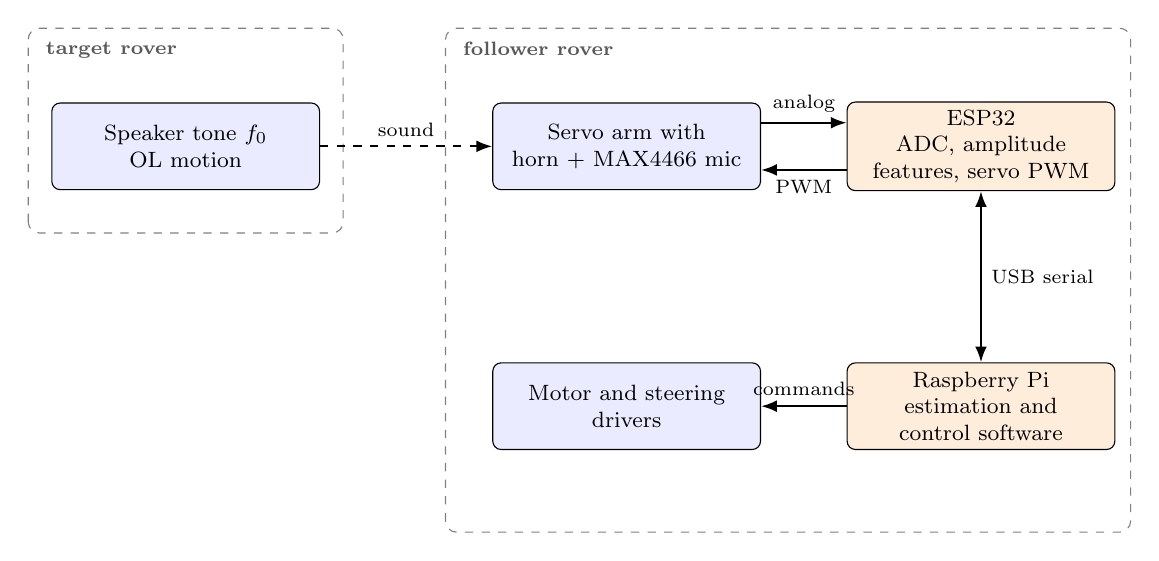
\begin{tikzpicture}[
  font=\footnotesize,
  blk/.style={draw, rounded corners=3pt, align=center, minimum height=11mm, minimum width=34mm, inner sep=3pt},
  hw/.style={blk, fill=blue!8},
  sw/.style={blk, fill=orange!14},
  link/.style={-{Latex[length=2mm]}, thick},
  both/.style={{Latex[length=2mm]}-{Latex[length=2mm]}, thick},
  snd/.style={-{Latex[length=2mm]}, thick, dashed},
  lbl/.style={font=\scriptsize, align=center},
  box/.style={draw, dashed, rounded corners=4pt, gray}
]
% ---- rover containers
\draw[box] (-0.4,-1.1) rectangle (3.6,1.5);
\node[lbl, anchor=north west, gray!70!black] at (-0.3,1.45) {\textbf{target rover}};
\draw[box] (4.9,-4.9) rectangle (13.6,1.5);
\node[lbl, anchor=north west, gray!70!black] at (5.0,1.45) {\textbf{follower rover}};
% ---- components
\node[hw] (tgt) at (1.6,0) {Speaker tone $f_0$\\OL motion};
\node[hw] (mic) at (7.2,0) {Servo arm with\\horn + MAX4466 mic};
\node[sw] (esp) at (11.7,0) {ESP32\\ADC, amplitude\\features, servo PWM};
\node[sw] (pi)  at (11.7,-3.3) {Raspberry Pi\\estimation and\\control software};
\node[hw] (drv) at (7.2,-3.3) {Motor and steering\\drivers};

% ---- links
\draw[snd] (tgt.east) -- node[above, lbl] {sound} (mic.west);
\draw[link] ([yshift=3mm]mic.east) -- node[above, lbl] {analog} ([yshift=3mm]esp.west);
\draw[link] ([yshift=-3mm]esp.west) -- node[below, lbl] {PWM} ([yshift=-3mm]mic.east);
\draw[both] (esp.south) -- node[right, lbl] {USB serial} (pi.north);
\draw[link] (pi.west) -- node[above, lbl] {commands} (drv.east);
\end{tikzpicture}%
}
\caption{System architecture: hardware components and communication links. Blue: physical elements; orange: computation. The signals and the control loop are shown in Fig.~\ref{fig:ctrl}.}
\label{fig:arch}
\end{figure}




The implemented system is a continuous nonlinear plant with sampled estimation and control and a discrete supervisory state. A local linear time-invariant (LTI) model supports gain design; the nonlinear simulator retains independent global poses, steering and speed lag, acceleration limits, and sequential acoustic captures. The controller receives simulated sensor packets through the same estimation interface used for recorded data. It has no access to simulated target truth.

The operating domain is planar motion on a flat indoor floor, a single known source, fixed source level, and low vehicle speeds. Range refers to the receiver--speaker reference points; chassis clearance is a separate geometric quantity. Speaker orientation, reflections, motor noise, and within-pair motion can violate the sensing assumptions. These effects require measured bounds before the simulation gains are transferred to the vehicles.

\begin{table}[t]
\caption{Nominal simulation assumptions; these are not measured hardware specifications.}
\label{tab:assumptions}
\centering\footnotesize
\begin{tabularx}{\columnwidth}{@{}Xr@{}}\toprule
Quantity & Value\\\midrule
Desired separation $d^\ast$ & $1.20\,\mathrm{m}$\\
Nominal speed $v_0$ & $0.18\,\mathrm{m/s}$\\
Wheelbase $L$ & $0.145\,\mathrm{m}$\\
Forward speed limits & $0.06$--$0.35\,\mathrm{m/s}$\\
Maximum steering magnitude & $25^\circ$\\
Speed / steering time constants & $0.25$ / $0.15\,\mathrm{s}$\\
Braking deceleration $a_b$ & $0.35\,\mathrm{m/s^2}$\\
Reference-point clearance / margin & $0.40$ / $0.10\,\mathrm{m}$\\
Assumed calibrated range domain & $0.55$--$3.50\,\mathrm{m}$\\
Horn width $\sigma$ / half-dither $\delta$ & $40^\circ$ / $20^\circ$\\\bottomrule
\end{tabularx}
\end{table}

\begin{table}[t]
\caption{Timing configuration and unresolved physical timing.}
\label{tab:timing}
\centering\footnotesize
\begin{tabularx}{\columnwidth}{@{}Xr@{}}\toprule
Quantity & Value / status\\\midrule
Control interval $T_s$ & $0.05\,\mathrm{s}$\\
Nominal pair period & $0.40\,\mathrm{s}$\\
Requested within-pair gap & $0.18\,\mathrm{s}$\\
Realized nominal simulated gap & $0.20\,\mathrm{s}$\\
Configured transport delay & $0.04\,\mathrm{s}$\\
Maximum accepted measurement age & $0.60\,\mathrm{s}$\\
Loss timeout / replay history & $1.30$ / $2.50\,\mathrm{s}$\\
Legacy static-log median pair period & $12.84\,\mathrm{s}$\\
Physical dwell, latency, jitter & \textcolor{red}{To measure}\\\bottomrule
\end{tabularx}
\end{table}
The simulator schedules captures and delivery on the $T_s$ grid. Thus the requested $0.18\,\mathrm{s}$ gap becomes $0.20\,\mathrm{s}$, and transport delivery is also quantized. A $20\,\mathrm{Hz}$ controller does not create $20\,\mathrm{Hz}$ acoustic information. The legacy static log contains five pairs, none usable, and cannot establish the required measurement rate.

\pending{H1 --- Hardware configuration}{Record measured wheelbase, reference-point offsets, steering calibration, motor deadband, speed map, actuator lag, braking response, speaker settings, and the final wiring/power arrangement. Replace assumed values only with traceable measurements.}


\section{Relative Kinematics and Local Design Model}
\subsection{Kinematic Analysis}
\label{sec:kinematic}
The follower (pose $(x_f,y_f,\theta_f)$, speed $v_f$) is front-steered with wheelbase $L$ and steering angle $\delta_s$, so $\omega_f=\tfrac{v_f}{L}\tan\delta_s$. The target has speed $v_t$ and yaw rate $\omega_t$. Fig.~\ref{fig:geom} clarifies the relative geometry used for range $\rho$, line-of-sight angle $\lambda$, bearing $\beta=\lambda-\theta_f$, relative heading $\varepsilon=\theta_t-\theta_f$, and aspect $\alpha=\theta_t-\lambda=\varepsilon-\beta$, such that
\begin{equation}
\begin{aligned}
\dot\rho&=v_t\cos\alpha-v_f\cos\beta,\\
\dot\beta&=\frac{v_t\sin\alpha+v_f\sin\beta}{\rho}-\omega_f,\\
\dot\varepsilon&=\omega_t-\omega_f.
\end{aligned}
\label{eq:nl}
\end{equation}

\begin{figure}[!t]
\centering
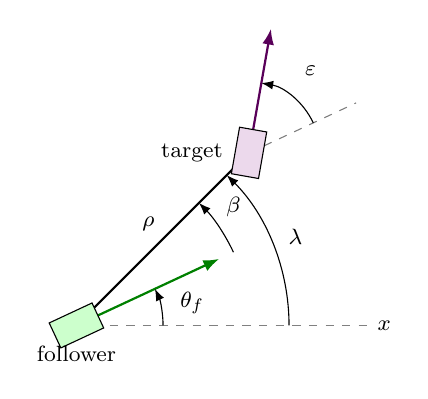
\begin{tikzpicture}[font=\footnotesize]
  \coordinate (F) at (0,0);
  \coordinate (T) at (45:3.1);
  \draw[gray, dashed] (F) -- (3.7,0) node[right, black] {$x$};
  \draw[gray, dashed] (T) -- ++(25:1.5);
  \draw[thick] (F) -- (T) node[midway, above left=-1pt] {$\rho$};
  \draw[-{Latex[length=2mm]}, thick, green!50!black] (F) -- ++(25:2.0);
  \draw[-{Latex[length=2mm]}, thick, violet!70!black] (T) -- ++(80:1.6);
  \node[draw, fill=green!20, rotate=25, minimum width=6mm, minimum height=3.5mm] at (F) {};
  \node[draw, fill=violet!15, rotate=80, minimum width=6mm, minimum height=3.5mm] at (T) {};
  \node[below=4pt] at (F) {follower};
  \node[left=6pt] at (T) {target};
  \draw[-{Latex[length=1.5mm]}] (1.1,0) arc (0:25:1.1);
  \node at (11:1.5) {$\theta_f$};
  \draw[-{Latex[length=1.5mm]}] (2.7,0) arc (0:45:2.7);
  \node at (22:3.0) {$\lambda$};
  \draw[-{Latex[length=1.5mm]}] (25:2.2) arc (25:45:2.2);
  \node at (37:2.5) {$\beta$};
  \draw[-{Latex[length=1.5mm]}, shift={(T)}] (25:0.9) arc (25:80:0.9);
  \node at ($(T)+(53:1.3)$) {$\varepsilon$};
\end{tikzpicture}
\caption{Relative geometry (green: follower, violet: target; arrows show velocity vectors): range $\rho$, bearing $\beta=\lambda-\theta_f$, relative heading $\varepsilon=\theta_t-\theta_f$.}
\label{fig:geom}
\end{figure}


\subsection{Linearization and Local LTI Model}
\label{sec:linearization}

To linearize the model, the nominal straight-line operating condition, where both rovers are moving in the same direction at the same speed while maintaining a constant separation, is considered with:
\[
\rho=d^\ast,\qquad
\beta=\varepsilon=0,\qquad
v_f=v_t=v_0>0,\qquad
\omega_f=\omega_t=0,
\]
where $d^\ast$ is the desired minimal separation between both vehicles and $v_0$ is the nominal forward speed.

The state vector, control input, disturbance from the target's motion, and measured output are then defined as
\[
\mathbf{x}=
\begin{bmatrix}
\delta\rho & \beta & \varepsilon
\end{bmatrix}^{\mathsf T},
\qquad
\mathbf{u}=
\begin{bmatrix}
\delta v_f & \omega_f
\end{bmatrix}^{\mathsf T},
\qquad
\mathbf{w}=
\begin{bmatrix}
\delta v_t & \omega_t
\end{bmatrix}^{\mathsf T},
\]
and
\[
\mathbf{y}=
\begin{bmatrix}
\hat{\rho}-d^\ast\\
\hat{\beta}
\end{bmatrix},
\]
where $\delta\rho=\rho-d^\ast$, $\delta v_f=v_f-v_0$, and $\delta v_t=v_t-v_0$. The relative heading is $\varepsilon=\theta_t-\theta_f$, and the bearing is $\beta=\lambda-\theta_f$. 

The measured outputs are the estimated range deviation $\hat{\delta\rho}$ and relative bearing $\hat{\beta}$ expressed relative to the follower's forward direction.

The control inputs are virtual commands: $\delta v_f$ represents a deviation from the nominal follower speed, while $\omega_f$ represents the commanded follower yaw rate. The target-motion variables $\delta v_t$ and $\omega_t$ are treated as disturbances because the follower does not directly know the target's real-time speed and yaw rate. \autoref{tab:model_variables} showcases the state space variables, their physical interpretation, and associated units. 

Linearizing the nonlinear relative-kinematics model about the nominal operating condition gives
\begin{equation}
\dot{\mathbf{x}}
=\mathbf{A}\mathbf{x}
+\mathbf{B}\mathbf{u}
+\mathbf{E}\mathbf{w},
\qquad
\mathbf{y}
=\mathbf{C}\mathbf{x}+\mathbf{n},
\label{eq:lin}
\end{equation}
where $\mathbf{n}$ represents measurement-estimation errors (to be determined experimentally). The measurement equation applies when a valid acoustic estimate becomes available; measurements are not assumed to arrive at every controller update.

For the constant-speed operating condition, the local model is LTI:
\begin{equation}
\begin{aligned}
\mathbf{A}
&=
\begin{bmatrix}
0&0&0\\
0&0&a\\
0&0&0
\end{bmatrix},
&
\mathbf{B}
&=
\begin{bmatrix}
-1&0\\
0&-1\\
0&-1
\end{bmatrix},\\[6pt]
\mathbf{E}
&=
\begin{bmatrix}
1&0\\
0&0\\
0&1
\end{bmatrix},
&
\mathbf{C}
&=
\begin{bmatrix}
1&0&0\\
0&1&0
\end{bmatrix},
\end{aligned}
\label{eq:mats}
\end{equation}
with
\[
a=\frac{v_0}{d^\ast}.
\]


Refer to Appendix \ref{app:der} for the supplementary derivations and to \autoref{fig:ctrl} for the block diagram. 

\begin{table*}[!t]
\centering
\caption{State-space variables and their physical interpretation.}
\label{tab:model_variables}
\small
\renewcommand{\arraystretch}{1.15}
\begin{tabular}{p{0.15\textwidth} p{0.10\textwidth} p{0.55\textwidth} p{0.10\textwidth}}
\hline
\textbf{Category} & \textbf{Variable} & \textbf{Physical meaning} & \textbf{Unit}\\
\hline
State
& $\delta\rho$
& Deviation of the actual follower-target distance  from the desired separation $d^\ast$
& m\\

State
& $\beta$
& Relative bearing of the target measured from the follower's forward direction
& rad\\

State
& $\varepsilon$
& Relative heading between the target and follower
& rad\\

Control input
& $\delta v_f$
& Deviation of the follower's forward speed from the nominal speed $v_0$
& m/s\\

Control input
& $\omega_f$
& Commanded yaw rate of the follower
& rad/s\\

Disturbance
& $\delta v_t$
& Deviation of the target's forward speed from the nominal speed $v_0$
& m/s\\

Disturbance
& $\omega_t$
& Target's yaw rate
& rad/s\\

Measured output
& $\hat{\rho}-d^\ast$
& Estimated range deviation obtained from the acoustic measurements
& m\\

Measured output
& $\hat{\beta}$
& Estimated relative bearing obtained from the acoustic measurements
& rad\\
\hline
\end{tabular}
\end{table*}

The range estimate is obtained from the amplitude model rather than from a direct distance measurement (\autoref{eq:rho}). 


\textbf{Separation convention.} In the retained formulation, ``desired minimal separation'' denotes the regulation setpoint $d^\ast$. The hard clearance $r_{\mathrm{clear}}$ is distinct and smaller. The output vector contains acoustic estimates; it is not a direct position measurement. The local matrices describe virtual speed/yaw inputs before actuator dynamics and saturation.
\begin{figure}[t]
\centering
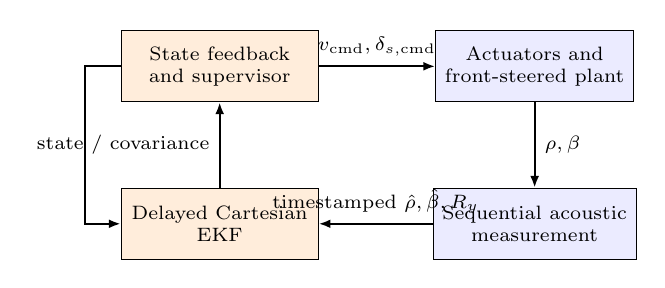
\begin{tikzpicture}[font=\scriptsize,
 b/.style={draw,align=center,minimum width=25mm,minimum height=9mm},
 a/.style={-{Latex[length=1.5mm]},thick}]
\node[b,fill=orange!14] (c) at (0,0) {State feedback\\and supervisor};
\node[b,fill=blue!8] (p) at (4,0) {Actuators and\\front-steered plant};
\node[b,fill=orange!14] (o) at (0,-2) {Delayed Cartesian\\EKF};
\node[b,fill=blue!8] (s) at (4,-2) {Sequential acoustic\\measurement};
\draw[a] (c) -- node[above] {$v_{\rm cmd},\delta_{s,\rm cmd}$} (p);
\draw[a] (p) -- node[right] {$\rho,\beta$} (s);
\draw[a] (s) -- node[above] {timestamped $\hat\rho,\hat\beta,R_y$} (o);
\draw[a] (o) -- node[left] {state / covariance} (c);
\draw[a] (c.west) -- ++(-.45,0) |- (o.west);
\end{tikzpicture}
\caption{Implemented output-feedback structure. The left return supplies commanded motion to the actuator predictor. The observer has no target-truth input; acoustic geometry is inferred from amplitude pairs.}
\label{fig:ctrl}
\end{figure}

\section{State-Space Analysis}
\label{sec:analysis}
\subsection{Realizations, Trajectories, and Stability}
For the retained local model, $a=v_0/d^\ast$ has units $\mathrm{s^{-1}}$ and $A^2=0$. Its state transition and constant-forcing response are
\begin{equation}
\begin{aligned}
\Phi(t,0)&=I+At,\\
\mathbf x(t)&=(I+At)\mathbf x(0)+\left(tI+\tfrac12t^2A\right)\mathbf f,
\end{aligned}
\label{eq:forced}
\end{equation}
where $\mathbf f=B\mathbf u+E\mathbf w$ is constant. With zero initial state, the input--output transfer matrix is
\begin{equation}
G(s)=C(sI-A)^{-1}B=
\begin{bmatrix}-1/s&0\\0&-(s+a)/s^2\end{bmatrix}.
\end{equation}
The range and bearing channels decouple in this local realization, although the nonlinear plant couples them. All open-loop eigenvalues are zero. For $a>0$, however, $\beta(t)=\beta(0)+at\varepsilon(0)$ under zero input. The nontrivial nilpotent Jordan block makes the equilibrium Lyapunov unstable. The transfer matrix is also not bounded-input bounded-output stable. Describing these poles as merely ``marginally stable'' would omit the Jordan structure.

State-space coordinates are not unique. For nonsingular $T$ and $\mathbf x=T\mathbf z$, the realization becomes $(T^{-1}AT,T^{-1}B,CT)$ without changing $G(s)$. For the bearing subsystem $[\beta,\varepsilon]^\top=T_b\mathbf z_b$, choose
\begin{equation}
T_b=\begin{bmatrix}-a&-1\\0&-1\end{bmatrix},\quad
A_c=\begin{bmatrix}0&1\\0&0\end{bmatrix},\quad
B_c=\begin{bmatrix}0\\1\end{bmatrix},\quad C_c=\begin{bmatrix}-a&-1\end{bmatrix}.
\end{equation}
This controllable canonical form is valid for $a>0$; its dual gives an observable canonical realization of the same scalar transfer function. The transformed coordinates carry the corresponding physical scaling. A diagonal eigenvector realization does not exist for the defective bearing block.

For the scheduled family $A(t)=a(t)N$, where $N_{23}=1$ and all other entries vanish, $N^2=0$ and the matrices commute. Consequently,
\begin{equation}
\Phi(t,s)=I+N\int_s^t a(\tau)\,\mathrm d\tau,
\end{equation}
\begin{equation}
\mathbf x(t)=\Phi(t,s)\mathbf x(s)+\int_s^t\Phi(t,\tau)\mathbf f(\tau)\,\mathrm d\tau.
\end{equation}
This is a specific linear time-varying (LTV) reference model. A varying nominal trajectory can introduce additional terms; the expression is not asserted for an arbitrary trajectory linearization.

\subsection{Controllability, Observability, and Partial Modes}
The controllability and observability matrices are $\mathcal C=[B,AB,A^2B]$ and $\mathcal O=[C^\top,(CA)^\top,(CA^2)^\top]^\top$. Their ranks depend on the operating point (Table~\ref{tab:ranks}). At $a>0$, the vector $AB_{(:,2)}=[0,-a,0]^\top$ supplies the third reachable direction, while $CA$ exposes the relative heading through the bearing derivative.

\begin{table}[t]
\caption{Local structural properties. Ranks are controllability / observability.}
\label{tab:ranks}\centering\footnotesize
\begin{tabularx}{\columnwidth}{@{}Xcc@{}}\toprule
Model & States & Ranks\\\midrule
Moving nominal plant, $a>0$ & 3 & 3 / 3\\
Stopped virtual-input plant, $a=0$ & 3 & 2 / 2\\
Plant with constant target disturbances & 5 & 3 / 5\\\bottomrule
\end{tabularx}
\end{table}

At $a=0$, the reachable subspace is $\operatorname{span}\{e_1,e_2+e_3\}$ and the unobservable subspace is $\operatorname{span}\{e_3\}$, with $e_i$ the standard basis vectors. The transformation $T_0=[e_1,e_2+e_3,e_3]$ separates a two-state controllable/observable block from an uncontrollable/unobservable zero mode. Neither state feedback nor an observer can move that hidden zero mode; the virtual-input model is not stabilizable or detectable. The physical vehicle is more restrictive because its yaw authority also vanishes at zero speed.

For constant target disturbances, define $\mathbf x_5=[\mathbf x^\top,\mathbf w^\top]^\top$ and
\begin{equation}
A_5=\begin{bmatrix}A&E\\0&0\end{bmatrix},\quad
B_5=\begin{bmatrix}B\\0\end{bmatrix},\quad C_5=\begin{bmatrix}C&0\end{bmatrix}.
\end{equation}
The two additional zero modes describe external target motion; follower commands do not control them. Their observability at $a>0$ permits disturbance estimation in the ideal linear model but does not prove practical identifiability under sparse, biased acoustic measurements.

\subsection{Numerical Checks and Local Validity}
Finite-difference Jacobians agree with $A$ and $B$ to maximum absolute errors $2.50\times10^{-14}$ and $1.00\times10^{-12}$ in the stored numerical coordinates. Forced LTI response, the commuting LTV transition, and transfer equivalence under similarity were independently checked against numerical integration or direct evaluation.

A three-second open-loop comparison starts from $\Delta\mathbf x=c[0.15\,\mathrm m,0.10\,\mathrm{rad},0.10\,\mathrm{rad}]^\top$. At $c=1$, maximum nonlinear--linear discrepancies are $0.00377\,\mathrm m$ in range and $0.00517\,\mathrm{rad}$ in bearing; at $c=2$, they increase to $0.01457\,\mathrm m$ and $0.01911\,\mathrm{rad}$. These finite tests illustrate local approximation error. They neither identify a region of attraction nor validate a model against a physical trajectory.

\section{Acoustic Measurement and State Estimation}
\label{sec:sensing}
\subsection{Calibrated Amplitude Model}
For mean-removed ADC samples $s[j]$, the tone amplitude is obtained from the discrete Fourier coefficient evaluated by a Goertzel recurrence \cite{goertzel}:
\begin{equation}
A=\frac{2}{N}\left|\sum_{j=0}^{N-1}s[j]e^{-\mathrm{i}2\pi f_0j/f_s}\right|.
\label{eq:goertzel}
\end{equation}
Here $N$ is the window length, $f_s$ the sampling frequency, and $f_0$ the tone frequency. Amplitude is expressed in ADC counts, not calibrated sound-pressure level. The assumed response is
\begin{equation}
A(\varphi)=K\rho^{-n}\exp\!\left[-\frac{(\varphi+b_0-\beta)^2}{2\sigma^2}\right]+\eta.
\label{eq:amp}
\end{equation}
The positive exponent $n$ describes range attenuation; $K$ has units of amplitude times $\mathrm{m}^{n}$; $b_0$ is the horn boresight offset; $\sigma$ is the angular width; and $\eta$ is additive amplitude error. All angular calculations use radians. A Gaussian response is a candidate local calibration model, not a consequence of horn geometry.

Let $A_\pm$ be positive, valid amplitudes acquired at actual commanded angles $\varphi_c\pm\delta$, with $\delta>0$. Neglecting scene changes during the pair gives
\begin{equation}
\hat\beta=\varphi_c+b_0+\frac{\sigma^2}{2\delta}\ln\frac{A_+}{A_-},
\label{eq:beta}
\end{equation}
\begin{equation}
\hat\rho=\left\{\frac{K}{\sqrt{A_+A_-}}
\exp\!\left[-\frac{(\varphi_c+b_0-\hat\beta)^2+\delta^2}{2\sigma^2}\right]\right\}^{1/n}.
\label{eq:rho}
\end{equation}
The amplitude ratio cancels a gain common to both captures. It does not cancel gain or range changes between captures. Absolute range remains confounded with source level: if the true amplitude constant is $gK$ while estimation uses $K$, then $\hat\rho=\rho g^{-1/n}$. Perfect regulation of estimated range gives
\begin{equation}
\rho_{\mathrm{eq}}=g^{1/n}d^\ast.
\label{eq:gainbias}
\end{equation}
Integral control cannot correct an unobserved calibration bias.

\subsection{Uncertainty and Calibration Acceptance}
Define $\ell_\pm=\ln A_\pm$, $c=\varphi_c+b_0$, and $k_\beta=\sigma^2/(2\delta)$. The Jacobian from $[\ell_+,\ell_-]^\top$ to $[\hat\rho,\hat\beta]^\top$ is
\begin{equation}
J=\begin{bmatrix}
\dfrac{\hat\rho}{n}\left(-\dfrac12+\dfrac{c-\hat\beta}{2\delta}\right)&
\dfrac{\hat\rho}{n}\left(-\dfrac12-\dfrac{c-\hat\beta}{2\delta}\right)\\[4pt]
k_\beta&-k_\beta
\end{bmatrix}.
\label{eq:covjac}
\end{equation}
The measurement covariance is $R_y=J\Sigma_\ell J^\top+R_{\mathrm{floor}}+R_{\mathrm{motion}}$. The first term retains range--bearing correlation. The remaining terms represent calibration/model error and bounded scene motion over the capture interval. Low amplitude amplifies logarithmic noise; clipped or invalid captures are rejected rather than assigned a nominal uncertainty.

The calibration program estimates $K,n,\sigma,b_0$ from explicitly supplied training recordings. Separate recordings test angular and distance coverage, fit residuals, repeatability, and timing. Files with identical content cannot appear in both sets. The commissioning gates are bearing RMSE at most $3^\circ$, relative range RMSE at most $10\%$, absolute bearing bias at most $2^\circ$, relative range bias at most $5\%$, valid-pair fraction at least $95\%$, and pair-period 95th percentile at most $0.5\,\mathrm{s}$. Validation requires at least three distances and five bearings, training log-amplitude RMSE at most $0.15$, and no fitted parameter at its optimization bound. These are proposed acceptance limits; no supplied physical calibration has passed them.

\pending{H2 --- Held-out acoustic calibration}{Insert fitted parameters with units, uncertainty and held-out errors; angular/range residual plots; clipping and rejection rates; source-aspect, motor-on, and room-repeatability trials. If the Gaussian/amplitude model fails, revise the sensing method and repeat the controller evaluation.}

\subsection{Cartesian Runtime Observer}
The local design state includes target heading, which is undefined for a stationary target. The runtime instead uses a \textbf{Cartesian constant-velocity extended Kalman filter} with
$\mathbf q=[p_x,p_y,v_{tx},v_{ty}]^\top$: relative position and target velocity, both resolved in the follower frame. For follower speed $v_f$ and yaw rate $\omega_f$,
\begin{equation}
\begin{aligned}
\dot p_x&=v_{tx}-v_f+\omega_f p_y,&\dot p_y&=v_{ty}-\omega_f p_x,\\
\dot v_{tx}&=\omega_f v_{ty},&\dot v_{ty}&=-\omega_f v_{tx}.
\end{aligned}
\label{eq:cartesian}
\end{equation}
Constant-input prediction uses the exact planar rotation and follower arc displacement. Isotropic white target-acceleration noise with spectral density $q_a$ contributes
\begin{equation}
Q_q=q_a\begin{bmatrix}\tfrac{\Delta t^3}{3}I_2&\tfrac{\Delta t^2}{2}I_2\\
\tfrac{\Delta t^2}{2}I_2&\Delta t I_2\end{bmatrix}.
\end{equation}
Here $q_a$ has units $\mathrm{m^2/s^3}$. The measurement function is
\begin{equation}
h(\mathbf q)=\begin{bmatrix}\sqrt{p_x^2+p_y^2}\\\operatorname{atan2}(p_y,p_x)\end{bmatrix}.
\end{equation}
Angular innovations are wrapped to $[-\pi,\pi)$. With innovation $\boldsymbol\nu$, Jacobian $H$, prior covariance $P^-$, and $S=HP^-H^\top+R_y$, a correction is accepted only if $\boldsymbol\nu^\top S^{-1}\boldsymbol\nu\le11.83$ and the sensor/domain checks pass. For Kalman gain $L_K=P^-H^\top S^{-1}$, the Joseph update is
\begin{equation}
P^+=(I-L_KH)P^-(I-L_KH)^\top+L_KR_yL_K^\top.
\end{equation}
The numerical gate is consistent with a two-dimensional Gaussian innovation model; reflections need not satisfy that distribution. Rejection statistics therefore remain part of the reported results.

Each pair is assigned its capture midpoint. A \textbf{delayed-measurement correction} restores the filter to that time, applies the update, and replays stored follower inputs to the present. Duplicate, reordered, or excessively old corrections are rejected. Rejected samples do not refresh the loss timer. Timestamp mapping unwraps the device clock and uses a minimum-offset estimate with a configured transport correction. Unknown constant transport delay and clock drift require measurement; this procedure is not a shared hardware clock.

Own-motion inputs come from the actuator model, not wheel odometry. Speed/steering calibration errors can therefore corrupt both prediction and control. The inferred relative heading is $\hat\varepsilon=\operatorname{atan2}(\hat v_{ty},\hat v_{tx})$ only above a target-speed threshold of $0.05\,\mathrm{m/s}$; otherwise the implementation uses zero heading feedback. Heading feedback is limited to $\pm45^\circ$. This is an implementation convention, not evidence that stationary target heading is observable.

\pending{H3 --- Dynamic estimation and time alignment}{Measure device/host delay, pair timing, drift over a trial, processing time and missed deadlines. Compare estimated range/bearing with independently timestamped reference trajectories, including stationary-follower and moving-follower tests. Report reference uncertainty and rejected updates.}

\section{Feedback Design and Supervisory Constraints}
\label{sec:control}
\subsection{Discrete Integral State Feedback}
\textbf{Linear quadratic integral (LQI) control} augments the local state with $\dot z=\rho-d^\ast$. For $\boldsymbol\xi=[\mathbf x^\top,z]^\top$,
\begin{equation}
A_a=\begin{bmatrix}A&0\\C_r&0\end{bmatrix},\quad
B_a=\begin{bmatrix}B\\0\end{bmatrix},\quad C_r=\begin{bmatrix}1&0&0\end{bmatrix}.
\end{equation}
Exact zero-order-hold discretization at $T_s$ uses a block exponential,
\begin{equation}
\exp\!\left(T_s\begin{bmatrix}A_a&B_a\\0&0\end{bmatrix}\right)
=\begin{bmatrix}A_d&B_d\\0&I_2\end{bmatrix}.
\end{equation}
This avoids inverting the singular matrix $A_a$. The nominal infinite-horizon cost is
\begin{equation}
J_c=\sum_{k=0}^{\infty}\left(\boldsymbol\xi_k^\top Q\boldsymbol\xi_k+\mathbf u_k^\top R\mathbf u_k\right).
\end{equation}
The diagonal weights are $Q=\operatorname{diag}(6,2,0.8,0.3)$ and $R=\operatorname{diag}(25,12)$ in the stated SI coordinate convention; their units are reciprocal to the squared state/input units, so each cost term is dimensionless. The integral state has units $\mathrm{m\,s}$. The Riccati equation and gain are
\begin{equation}
\begin{aligned}
P_R&=A_d^\top P_RA_d+Q\\
&\quad-A_d^\top P_RB_d(R+B_d^\top P_RB_d)^{-1}B_d^\top P_RA_d,\\
K_c&=(R+B_d^\top P_RB_d)^{-1}B_d^\top P_RA_d.
\end{aligned}
\end{equation}
The virtual command is $\mathbf u_k=-K_c[\hat\rho-d^\ast,\hat\beta,\hat\varepsilon,z]^\top$. For Table~\ref{tab:assumptions}, the numerical gain is
\begin{equation}
K_c\simeq\begin{bmatrix}
-0.668891&0&0&-0.107705\\
0&-0.402206&-0.186979&0
\end{bmatrix}.
\end{equation}
The negative range coefficients are consistent with $\dot{\delta\rho}=-\delta v_f+\delta v_t$: a positive range error must increase forward speed. Gains are simulation values pending identification.

For the ideal unconstrained full-state discrete loop $F=A_d-B_dK_c$, the poles are approximately $0.977032$, $0.979657$, $0.986764$, and $0.993433$. A discrete Lyapunov solution satisfies
\begin{equation}
F^\top P_LF-P_L=-I_4,\qquad P_L\succ0,
\end{equation}
with minimum eigenvalue $16.3695$ and maximum absolute residual $1.42\times10^{-14}$ in these coordinates. Thus this local reference is asymptotically stable. The certificate excludes saturation, asynchronous estimation, actuator lag, and supervisory switching.

The design discretizes the ideal augmented dynamics exactly. Runtime integration uses a forward-Euler update with anti-windup:
\begin{equation}
z_{k+1}=\sat_{[-z_{\max},z_{\max}]}\left\{z_k+T_s\left[e_k+\frac{v_k-v_{\mathrm{des},k}}{k_iT_{\mathrm{aw}}}\right]\right\},
\end{equation}
where $e_k=\hat\rho_k-d^\ast$, $k_i=-K_{c,14}$, $T_{\mathrm{aw}}=1\,\mathrm s$, $z_{\max}=3\,\mathrm{m\,s}$, and $v_k$ is the realizable forward command. Consequently, the ideal poles are not the eigenvalues of every runtime operating mode. The simulations evaluate the implemented update.

\subsection{Comparisons and Output Feedback}
The \textbf{pole-placement controller} assigns the range/integral pair to $\exp\{[-0.30,-0.45]T_s\}$ and the bearing/heading pair to $\exp\{[-0.35,-0.50]T_s\}$, with continuous pole parameters in $\mathrm{s^{-1}}$. Channel-wise assignment makes one explicit choice among the nonunique MIMO feedback gains. Alternative gains with the same eigenvalues can change eigenvectors, input effort, coupling, and sensitivity.

The \textbf{bearing-only steering baseline} commands $v_{\mathrm{des}}=0.22\,\mathrm{m/s}$ and $\omega_{\mathrm{des}}=0.6\hat\beta\,\mathrm{s^{-1}}$. It shares sensing, estimation, speed limits, and the range-dependent supervisor with the other methods. Its tracking law has no range regulator; the complete baseline is therefore not a purely bearing-only sensing system. Shared stopping logic prevents an unfair comparison against an unconstrained constant-speed vehicle.

In the ideal synchronous linear output-feedback reference, coordinates $[\boldsymbol\xi^\top,\tilde{\mathbf x}^\top]^\top$ yield a block upper-triangular closed-loop matrix with diagonal blocks $F$ and $F_e=(I-L_oC)A_{d,3}$. Here $A_{d,3}$ is the discretized three-state plant, $L_o$ a linear correction gain, and $\tilde{\mathbf x}$ the estimation error. The eigenvalues are the union of controller and observer-error poles. This separation-principle check does not establish stability for the delayed nonlinear EKF and switched constrained controller.

\subsection{Feasible Commands and Terminal Approach}
Forward speed is clipped to the configured maximum and braking bound, reduced by $\max\{0.25,\cos^2\hat\beta\}$, and set to zero below the motor deadband. The yaw command obeys
\begin{equation}
|\omega_f|\le\frac{v_f}{L}\tan\delta_{s,\max},\qquad
\delta_s=\arctan\!\left(\frac{L\omega_f}{v_f}\right),\quad v_f>0.
\end{equation}
At zero speed, both commanded yaw and steering are set to zero. Reverse motion is excluded.

Following and stationary-source approach are distinct missions. The operator must explicitly select the stationary mission, which initializes a zero target-velocity prior and uses $v_{\mathrm{des}}=0.8(\hat\rho-d^\ast)\,\mathrm{s^{-1}}$ and $\omega_{\mathrm{des}}=1.0\hat\beta\,\mathrm{s^{-1}}$. A terminal band accounts for braking distance and motor deadband, then latches the stop. This shared approach mode is used under every controller label; its results cannot demonstrate an LQI advantage at a stationary equilibrium.

\subsection{Supervision and Conditional Stopping Bound}
In ACQUIRE, the chassis remains stationary until three accepted observations pass the estimator and acquisition checks. Rejected packets do not count, but do not necessarily reset the accepted-pair counter. TRACK applies feedback. Stale measurements, excessive covariance, or a bearing outside $\pm55^\circ$ produce recoverable HOLD. A near-target mean range or the explicit terminal condition produces latched STOP. Horn scanning enables reacquisition while the vehicle is stopped.

The speed limiter imposes
\begin{equation}
v_fT+\frac{v_f^2}{2a_b}\le
\hat\rho-3\sigma_\rho-r_{\mathrm{clear}}-m,
\label{eq:brake}
\end{equation}
where $T$ is the loss timeout plus speed lag, $a_b>0$ the assumed braking deceleration, $\sigma_\rho$ the estimated range standard deviation, $r_{\mathrm{clear}}$ the reference-point clearance, and $m$ an additional margin. Every term has units of distance. A negative right-hand side blocks motion. The bound presumes a meaningful uncertainty interval, a valid braking model, and a nonapproaching target. It cannot prevent a target from driving into the follower or detect an obstacle outside the acoustic measurement.

A separate motor process stops when the controller heartbeat expires. This covers a stalled control process while the motor process and driver remain responsive; it does not cover a frozen operating system, blocked motor bus, or failed driver. Physical trials require a separate motor power cut.

\pending{H4 --- Physical constraints and watchdog}{Measure stopping distance at several speeds, heartbeat response, driver stop behavior, steering/speed saturation, and recovery after missing packets. State the measured domain in which the stopping bound is credible.}

\section{Validation Protocol and Simulation Results}
\label{sec:valid}
\subsection{Evidence and Performance Definitions}
The authoritative comparison, generated on 15 November 2026, contains $432$ simulated trials: three controller labels, twelve scenarios, and twelve seeds ($3000$--$3011$). Each trial lasts $60\,\mathrm s$. Initial range is sampled uniformly from $d^\ast+[0.25,0.45]\,\mathrm m$, bearing from $[-15^\circ,15^\circ]$, and relative heading from $[-5^\circ,5^\circ]$. The same scenario and seed schedule is used for each method. Saved configurations, source snapshots, hashes, per-trial metrics, and seed-$3000$ traces identify the evaluated implementation. A separate sensitivity study contains $78$ trials with seeds $4000$--$4005$.

\textbf{All closed-loop results in this section are synthetic.} The acoustic generator and estimator share the same response family, except for the specified perturbations. The trials assess implementation behavior under stated assumptions; they cannot validate the actual horn response or room acoustics. The $26$ saved Python tests cover model calculations, calibration rejection, protocol handling, delayed correction, supervision, and software motor-heartbeat behavior. They do not exercise physical motors or ADC acquisition.

Let $e_i=\rho_i-d^\ast$ and let $\mathcal T$ contain the last ten seconds of a run. Reported tail metrics are
\begin{equation}
\bar e=\frac{1}{|\mathcal T|}\sum_{i\in\mathcal T}e_i,\quad
e_{\mathrm{RMS}}=\sqrt{\frac{1}{|\mathcal T|}\sum_{i\in\mathcal T}e_i^2},
\end{equation}
and the analogous bearing RMS. A practical tracking pass requires $|\bar e|\le0.15\,\mathrm m$, bearing RMS $\le10^\circ$, TRACK occupancy at least $70\%$ over the full trial, and no simulated clearance violation. The mean-error gate is not an RMSE gate: a run can meet it despite substantial fluctuations. Aggregated RMSE includes every seed, including failed trials.

The original transient objective is retained separately: $2\%$ settling within $6\,\mathrm s$ and overshoot at most $15\%$. The saved implementation defines the settling band as $0.02|e_0|$, requires all subsequent samples to remain inside it, and measures time from trial start, including acquisition. For the positive initial errors used here, overshoot is $100\max\{0,-\min_i e_i\}/|e_0|$. No post-step time origin is introduced for the speed-change scenario. This convention is strict under noise and should not be confused with a fitted dominant-pole settling estimate.

\begin{table*}[t]
\centering\footnotesize
\caption{Controller comparison over twelve seeds per scenario. Each cell gives practical tracking passes / mean tail range RMSE in metres. All outcomes, including failures, enter the mean.}
\label{tab:comparison}
\begin{tabular}{@{}lccc@{}}\toprule
Scenario & LQI & Pole placement & Bearing-only steering\\\midrule
Nominal following & 12/12 / 0.0041 & 12/12 / 0.0043 & 0/12 / 0.1697 \\
Target speed increase & 12/12 / 0.0041 & 12/12 / 0.0043 & 0/12 / 0.2651 \\
Gentle turn & 12/12 / 0.0044 & 12/12 / 0.0045 & 0/12 / 0.1698 \\
Actuator mismatch & 12/12 / 0.0036 & 12/12 / 0.0038 & 0/12 / 0.8086 \\
Five-second signal loss & 12/12 / 0.0043 & 12/12 / 0.0044 & 1/12 / 0.1577 \\
Noise, drops, amplitude outliers, jitter & 11/12 / 0.1210 & 11/12 / 0.1206 & 10/12 / 0.7447 \\
Source gain $+20\%$ & 0/12 / 0.2412 & 0/12 / 0.2413 & 12/12 / 0.0363 \\

\bottomrule\end{tabular}
\end{table*}

\subsection{Regulation and Disturbance Response}
Both integral controllers pass all twelve nominal straight-following trials, the $0.05\,\mathrm{m/s}$ target-speed increase at $20\,\mathrm s$, the gentle turn, the actuator mismatch, and the five-second signal outage. The turn applies target yaw rate $0.025\,\mathrm{rad/s}$ between $15$ and $40\,\mathrm s$; actuator mismatch scales realized speed by $0.8$ and both lag constants by $1.7$. These perturbations are selected test conditions, not estimated physical distributions.

Nominal LQI mean tail range RMSE is $0.00409\,\mathrm m$, with worst-seed bearing RMS $0.545^\circ$. The constant-speed baseline passes none of the nominal trials and has mean tail range RMSE $0.170\,\mathrm m$. Its small bearing error does not imply distance regulation. Pole placement produces similar tracking outcomes to LQI; the present experiment supports both designs and does not establish statistical superiority of either.

\begin{figure*}[t]
\centering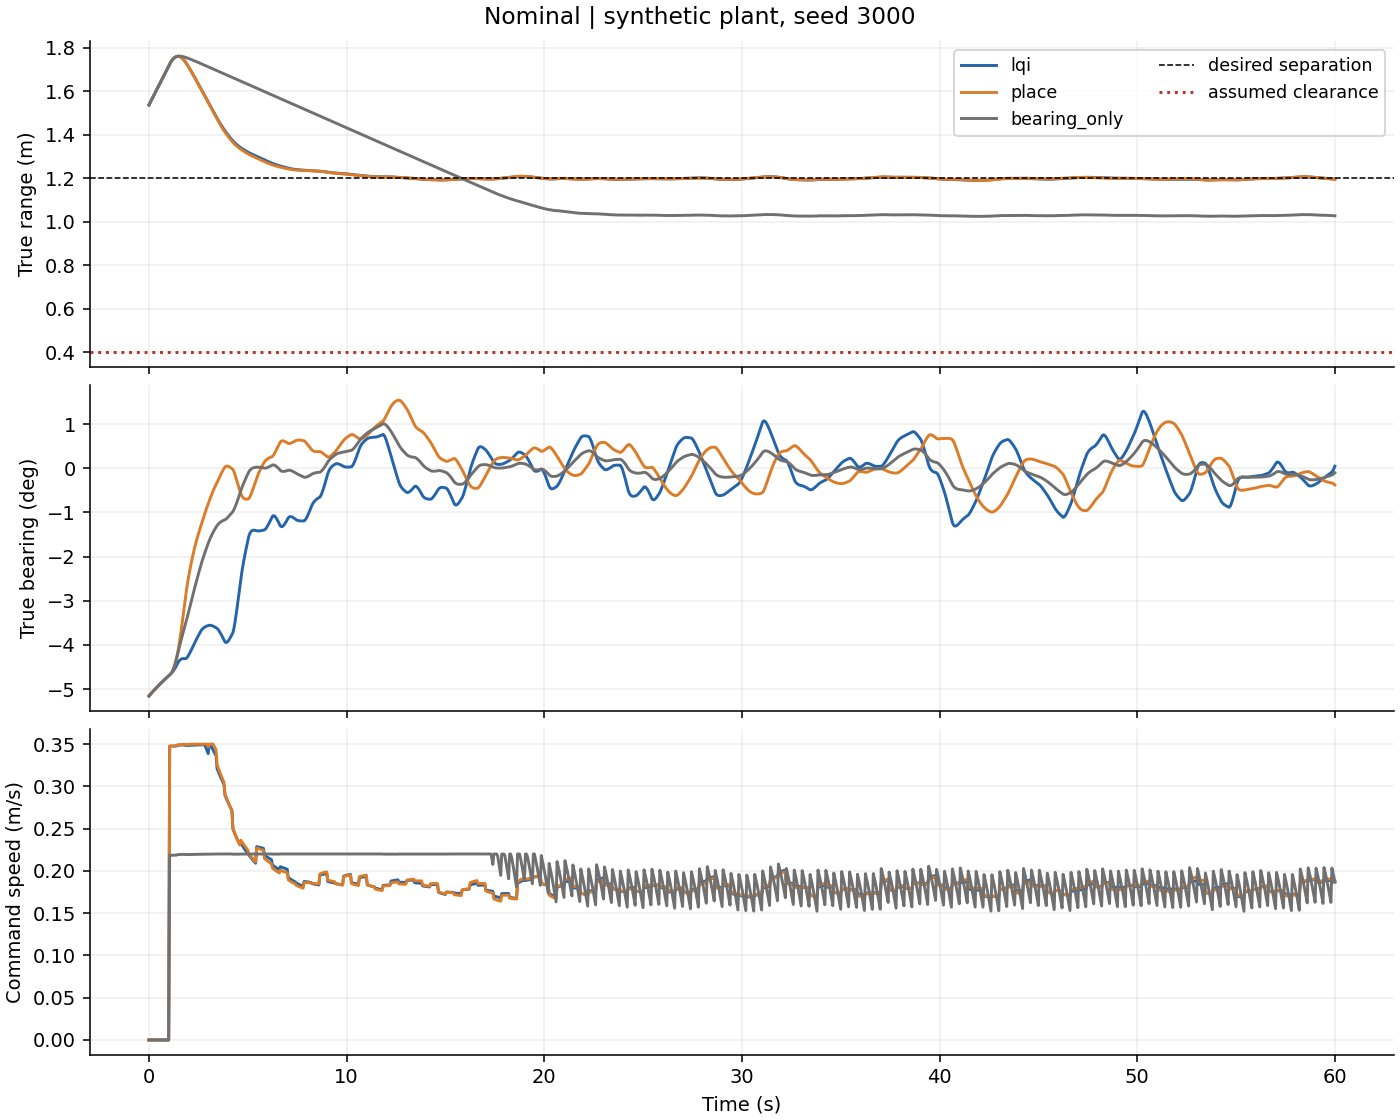
\includegraphics[width=0.88\textwidth]{figures/nominal.png}
\caption{Nominal synthetic response for seed $3000$, copied from the authoritative comparison run. The twelve-seed aggregates, rather than this example trace alone, determine reported pass counts.}
\label{fig:nominal}
\end{figure*}

In the combined stress case, additive amplitude noise doubles, packet-drop probability is $0.15$, independent amplitude perturbations occur on $12\%$ of pairs, and requested pair intervals vary by up to $15\%$. The amplitude perturbation is a synthetic reflection proxy, not a wave-propagation model. LQI and pole placement each pass $11/12$ trials; LQI mean tail range RMSE is $0.121\,\mathrm m$ and worst-seed bearing RMS is $3.11^\circ$. The baseline passes $10/12$ by the mean-error criterion but has mean RMSE $0.745\,\mathrm m$, illustrating why pass counts alone are insufficient.

The outage from $18$ to $23\,\mathrm s$ forces stopping and subsequent stationary reacquisition. Both integral designs recover under the modeled conditions. Neither result removes the need to measure loss-detection and motor-stop latency.

\begin{figure*}[t]
\centering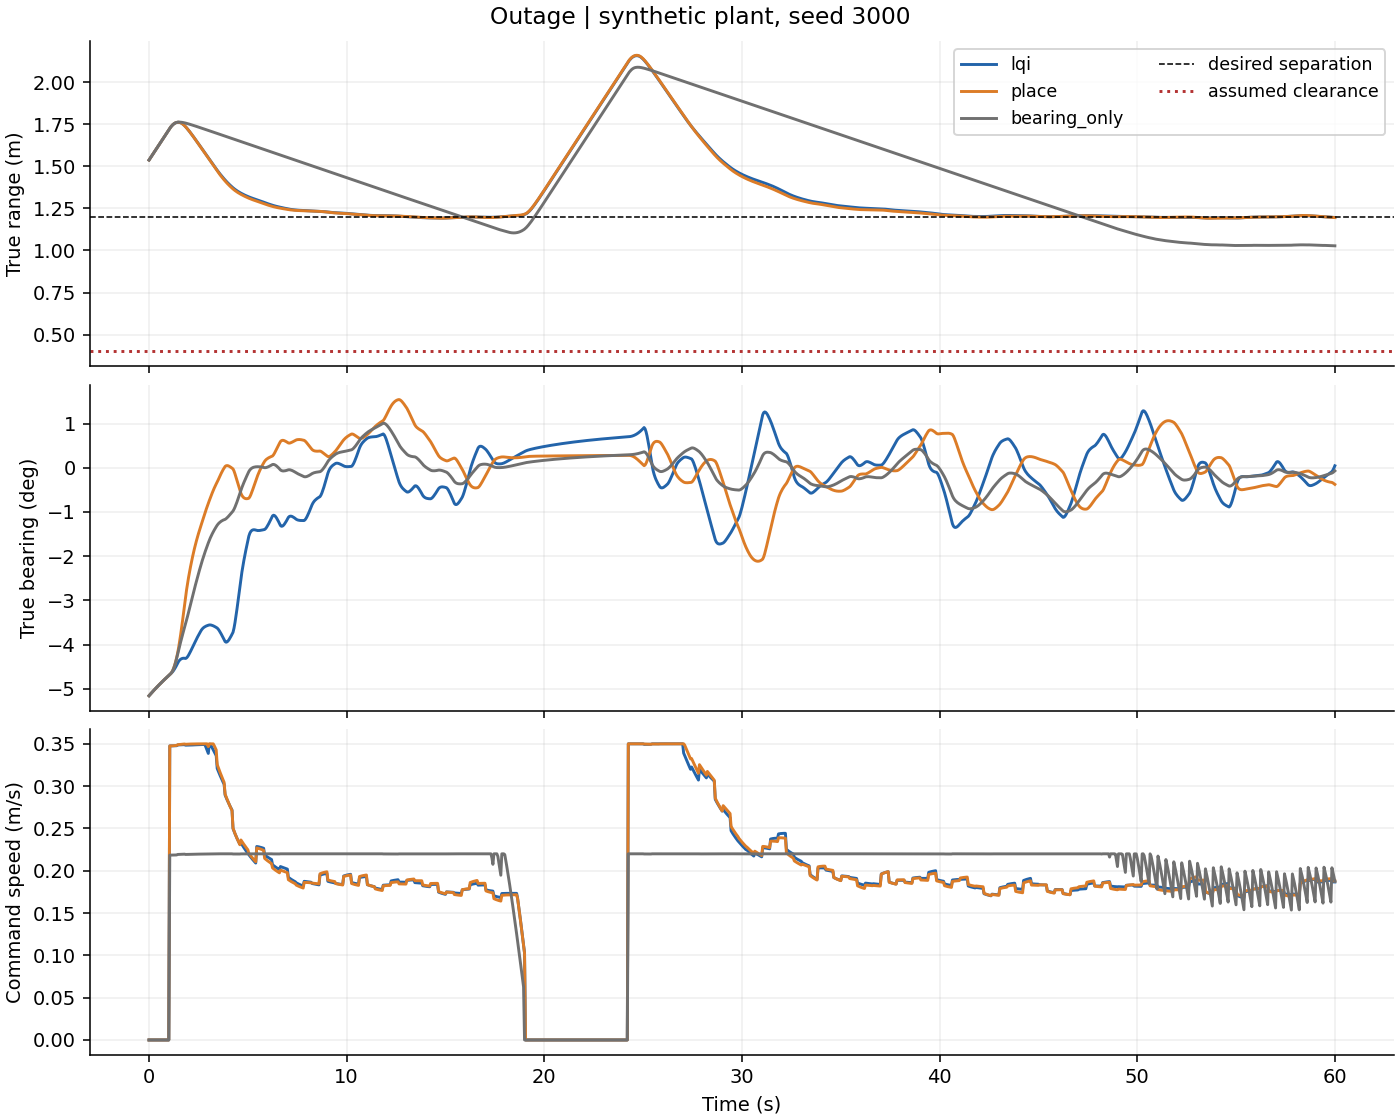
\includegraphics[width=0.88\textwidth]{figures/outage.png}
\caption{Synthetic five-second signal interruption, seed $3000$. State estimates, commands, and vehicle response are evaluated with the acquisition/hold logic active.}
\label{fig:outage}
\end{figure*}

\subsection{Failure Cases and Separate Terminal Tests}
A common source-level increase of $20\%$ produces LQI tail range RMSE $0.241\,\mathrm m$ and zero practical tracking passes. With $n=1$, Eq.~\eqref{eq:gainbias} predicts a true equilibrium shift of $0.2d^\ast=0.24\,\mathrm m$, consistent with the simulation. Integral action regulates the biased estimate. The baseline's $12/12$ passes in this single biased scenario result from its shared constraints and particular trajectory; they do not demonstrate rejection of arbitrary gain drift.

No-source trials and the $1.2\,\mathrm s$ and $12.84\,\mathrm s$ pair-period cases command zero motion in all twelve LQI trials. These are successful motion-inhibition tests, not tracking successes. A target at $0.50\,\mathrm{m/s}$ exceeds the follower's configured $0.35\,\mathrm{m/s}$ speed limit and cannot be followed at the desired separation. Its tracking failures are retained.

The explicitly declared stationary-source mission passes its separate standoff metric in $12/12$ trials under each controller label. This metric checks final-ten-second absolute mean range error at most $0.15\,\mathrm m$ and clearance; it does not independently test stop-latch activation. For LQI-labeled runs, mean final-ten-second range error is approximately $+0.060\,\mathrm m$, worst bearing RMS is $2.74^\circ$, and minimum range is $1.243\,\mathrm m$. These results concern the shared proportional terminal controller. Stop-latch behavior must also be checked in the command/mode history. Applying the moving-tracking occupancy criterion would incorrectly penalize an intended final stop.

No configured clearance violation occurs in the $432$ comparison trials or the $78$ sensitivity trials. This statement refers only to the modeled reference-point clearance. It is not an experimental collision-avoidance guarantee.

\subsection{Sensitivity to Measurement Assumptions}
With correct calibration in both generator and estimator, increasing Gaussian width $\sigma$ from $25^\circ$ to $160^\circ$ increases worst-seed tail bearing RMS from $0.329^\circ$ to $7.44^\circ$; all six trials at each width pass. A broad response reduces differential amplitude information. This sweep tests sensitivity under the assumed amplitude level, not the actual horn's shape or available signal-to-noise ratio.

Requested capture gaps of $0.10$, $0.18$, and $0.30\,\mathrm s$ pass six trials each. A $0.50\,\mathrm s$ gap with a $1.0\,\mathrm s$ pair period fails all six, with mean tail range RMSE approximately $0.177\,\mathrm m$. Raising control frequency cannot undo within-pair motion error. Additive amplitude-noise sweeps from $0.2$ to $5$ counts pass under the assumed $K=100$ amplitude calibration; these absolute noise values are not transferable to another gain setting.

\subsection{Robustness Analysis and Unmet Objectives}
A separate local periodic reference includes actuator lag, intermittent linear-observer corrections, exact delayed replay, and an Euler integral state. Its monodromy matrix is the product of the step maps over one measurement period; local stability requires every eigenvalue to lie inside the unit circle. The tested periods are $\{0.2,0.4,0.8,1.2\}\,\mathrm s$, delays $\{0,0.1,0.3\}\,\mathrm s$, and feedback-gain multipliers $\{0.5,1,2\}$. All $33$ valid combinations with delay shorter than the period are stable; the remaining three combinations are excluded by the reference formulation.

This reference assumes known realized actuator forcing in the predictor and exact replay. Its weak sensitivity to delay is conditional on those assumptions. The runtime uses modeled own motion and nonlinear measurements, and can fail an acquisition or performance criterion even when the local periodic reference is stable. The sweep does not establish the progress report's proposed $45^\circ$ phase margin or $6\,\mathrm{dB}$ gain margin.

The current LQI tuning meets the original joint settling/overshoot target in none of the nominal trials. The practical tail criterion is an explicitly revised commissioning metric, not evidence that the original transient target was achieved. Physical tuning and any revised specification must be justified using measured sensing delay, noise, motor deadband, and steering authority.

\begin{table}[t]
\caption{Disposition of the progress-report objectives.}
\label{tab:spec}\centering\footnotesize
\begin{tabularx}{\columnwidth}{@{}lX@{}}\toprule
ID & Current interpretation and evidence\\\midrule
O1 & Integral rejection of constant speed mismatch is local and conditional on calibration and feasible actuation; true-range bias persists under gain error.\\
O2 & Original bearing RMS limits: $10^\circ$ stationary, $20^\circ$ moving. The practical simulation gate uses the stricter $10^\circ$ moving limit.\\
O3 & Original $2\%$ settling $\le6\,\mathrm s$ and overshoot $\le15\%$: not achieved jointly by nominal LQI.\\
O4 & Configured limits and clearance checked in simulation. Physical stopping and clearance remain unverified.\\
O5 & Periodic local stability sweep completed. Original $45^\circ$ phase / $6\,\mathrm{dB}$ gain margins remain unverified.\\\bottomrule
\end{tabularx}
\end{table}

\pending{V1 --- Final robustness and transient claims}{After physical identification, rerun the simulations with the measured configuration; report original O1--O5 outcomes, transient distributions and failures. If classical margins are retained, define the loop break, delayed linearized model and treatment of the other channel. Otherwise explicitly revise the robustness objective.}

\section{Experimental Validation}
\label{sec:hardexp}
\subsection{Available Measurements}
The preliminary directional test is retained in Appendix~\ref{app:poc}. It compares eight angular positions at $0.30\,\mathrm m$ and supports a coarse orientation-dependent response. It does not establish a local Gaussian slope at the operating tone, range accuracy over the tracking domain, or the paired-measurement update rate.

The supplied static recording dated 22 October 2026 contains five packets with median pair period $12.84\,\mathrm s$, zero accepted measurements, and zero nonzero commands in offline replay. Three silence recordings contain two packets each and no valid measurements. These records demonstrate the current data limitation and the software's refusal to move on unusable data. They do not demonstrate closed-loop tracking.

\subsection{Hardware Identification and Sensing}
\pending{E1 --- Bench identification}{Insert final sensor calibration and actuator identification from H1--H4. Give trial dates, firmware/configuration versions, sample counts, training versus held-out split, reference instruments, and measurement uncertainties. Include distance/angle grids, source orientation, motor-on noise, and pair-timing distributions.}

\subsection{Moving-Target Following}
\pending{E2 --- Straight following and speed change}{Run repeatable marked trajectories with independently recorded target/follower references. Report range/bearing errors, settling/overshoot with stated time origin, control effort, saturation, TRACK/HOLD occupancy, minimum clearance, timing, and every failed trial. Compare LQI, pole placement, and the shared-supervisor baseline using the same calibrated limits.}

\pending{E3 --- Turning and Signal Loss}{Measure feasible turning trajectories, a controlled source interruption, reacquisition delay, and the effect of target/speaker aspect. Include synchronized trajectory plots and logs. Keep the target within demonstrated speed and curvature limits.}

\subsection{Stationary Approach and Model Agreement}
\pending{E4 --- Terminal approach}{Test the explicitly selected stationary mission separately from moving-target regulation. Report terminal separation distribution, braking distance, stop latch behavior, and motor-deadband effects.}

\pending{E5 --- Model versus hardware}{Compare measured small-perturbation trajectories with the local LTI prediction and the identified nonlinear simulation, using matched initial conditions and commands. Quantify prediction errors and the domain over which the model is useful. A tape-marked path needs a timestamped position/heading reference; an IMU alone is not position ground truth.}

\section{Discussion and Limitations}
The nominal design is controllable and observable only within its moving operating regime. At rest, loss of heading information coincides with loss of steering authority. The separate terminal mission avoids claiming that the same LQI equilibrium applies to both moving pursuit and stationary arrival.

The principal unresolved limitation is acoustic range identifiability. A multiplicative source or receiver gain change is indistinguishable from range under Eq.~\eqref{eq:amp}. The simulated bias test exposes this ambiguity directly. Recalibration and fixed source settings can reduce drift, but only held-out measurements can establish an acceptable operating domain. If amplitude range is not repeatable, the project needs an additional observable quantity or a revised task; controller retuning alone is insufficient.

Sequential sensing introduces another constraint. The two amplitudes correspond to different positions and orientations. Covariance inflation accounts for bounded mismatch, while delayed replay accounts for measurement age; neither reconstructs information lost through an invalid measurement model. The fixed-rate control loop also runs on a non-real-time operating system. Measured scheduling delay, clock drift, and transport uncertainty must therefore accompany any claim about bandwidth or recovery time.

The observer predicts follower motion without encoder feedback. Motor deadband, slip, battery voltage, and load can bias that prediction. Existing actuator stress tests cover only selected scale and lag errors. Similarly, synthetic reflection events do not cover persistent multipath, several sources, non-Gaussian ambiguity, or source occlusion. No global convergence or arbitrary-obstacle guarantee is asserted.

The demonstrated contribution at this stage is a reproducible connection between a relative state-space model, realizable front-steered feedback, delayed acoustic estimation, and explicit failure tests. The experimental contribution remains open until sensing accuracy, actuator behavior, and closed-loop following have been measured.

\pending{D1 --- Discussion from measured evidence}{Explain where the measured model agrees or fails, whether integral control improves distance regulation over the baseline, which constraint limits bandwidth, and which conclusions survive changes in source aspect and room conditions. Avoid generalizing beyond the tested domain.}

\section{Conclusion}
The moving-target local model admits observable and controllable state feedback, whereas the stopped vehicle requires a separate terminal treatment. Discrete LQI and channel-wise pole placement regulate simulated following distance under the nominal conditions and selected disturbances; a constant-speed bearing steering law does not. Calibration bias and slow sequential capture remain decisive limitations. The software and simulation evidence supports proceeding to gated hardware trials, but does not yet establish a successful physical tracking system.

\pending{C1 --- Final experimental conclusion}{Replace this provisional conclusion after E1--E5: state measured tracking/terminal accuracy, operating speed and sensing rate, comparative controller results, failed objectives, and the validated operating domain. Update the abstract consistently.}


\bibliographystyle{IEEEtranN}
\bibliography{refs}

\appendices
\section{Reproducibility and Evidence Status}
The repository is \href{https://github.com/helenejabbour/Audio-Tracking-Rover}{Audio-Tracking-Rover}. The local evidence archive dated 15 November 2026 contains the comparison run \texttt{20261115T163143\_844160Z\_validation}, sensitivity run \texttt{20261115T163216\_183097Z\_sensitivity}, and static-log replay \texttt{20261115T162526\_373664Z\_replay}. These directories preserve configurations, source snapshots, seed-specific metrics, and test output. The implementation is in \texttt{rover/}; the synthetic parameter file is \texttt{Config/simulation.json}. Archived development runs are not used as final evidence.

The ESP32 V2 firmware build was blocked before compilation by a Windows compiler startup failure. The independent MATLAB reference could not execute because the licensing service was unavailable. Neither is described as validated. The legacy Simulink model is retained but is not the source of the reported Python results.
\pending{R1 --- Reproducible final release}{Insert successful ESP32 build and board test, MATLAB cross-check if executed, final repository commit/release, measured configuration, raw hardware logs, and dated run identifiers. Update toolchain status without deleting the record of earlier failed attempts.}

\section{Supplementary Derivations}
\label{app:der}
\subsection{Linearization}
Let $f_1=v_t\cos\alpha-v_f\cos\beta$, $f_2=(v_t\sin\alpha+v_f\sin\beta)/\rho-\omega_f$, $f_3=\omega_t-\omega_f$. At the nominal point ($\alpha=\beta=0$, $\rho=d^\ast$, $v_t=v_f=v_0$): $\partial f_1/\partial v_t=1$, $\partial f_1/\partial v_f=-1$, with all other partials of $f_1$ zero; $\partial f_2/\partial\alpha=\partial f_2/\partial\beta=v_0/d^\ast=a$, $\partial f_2/\partial\omega_f=-1$, all other partials zero. Using $\alpha+\beta=\varepsilon$ gives $\delta f_2=a\varepsilon-\omega_f$, which yields \eqref{eq:mats}.


\subsection{Pairwise Inversion}
With $c=\varphi_c+b_0$, subtracting the two noiseless log-amplitude equations gives $\ln A_+-\ln A_-=2\delta(\beta-c)/\sigma^2$. Averaging gives $\tfrac12\ln(A_+A_-)=\ln K-n\ln\rho-[(c-\beta)^2+\delta^2]/(2\sigma^2)$, in the fixed amplitude/metre numerical convention. These relations yield Eqs.~\eqref{eq:beta}--\eqref{eq:rho}; differentiating them yields Eq.~\eqref{eq:covjac}.

\section{Proof of Concept}
\label{app:poc}
A proof of concept (POC) was conducted to evaluate the extent to which the MAX4466 microphone can detect a change in distance or orientation of the emitted sound. 

\begin{figure}[ht!]
\begin{center}
    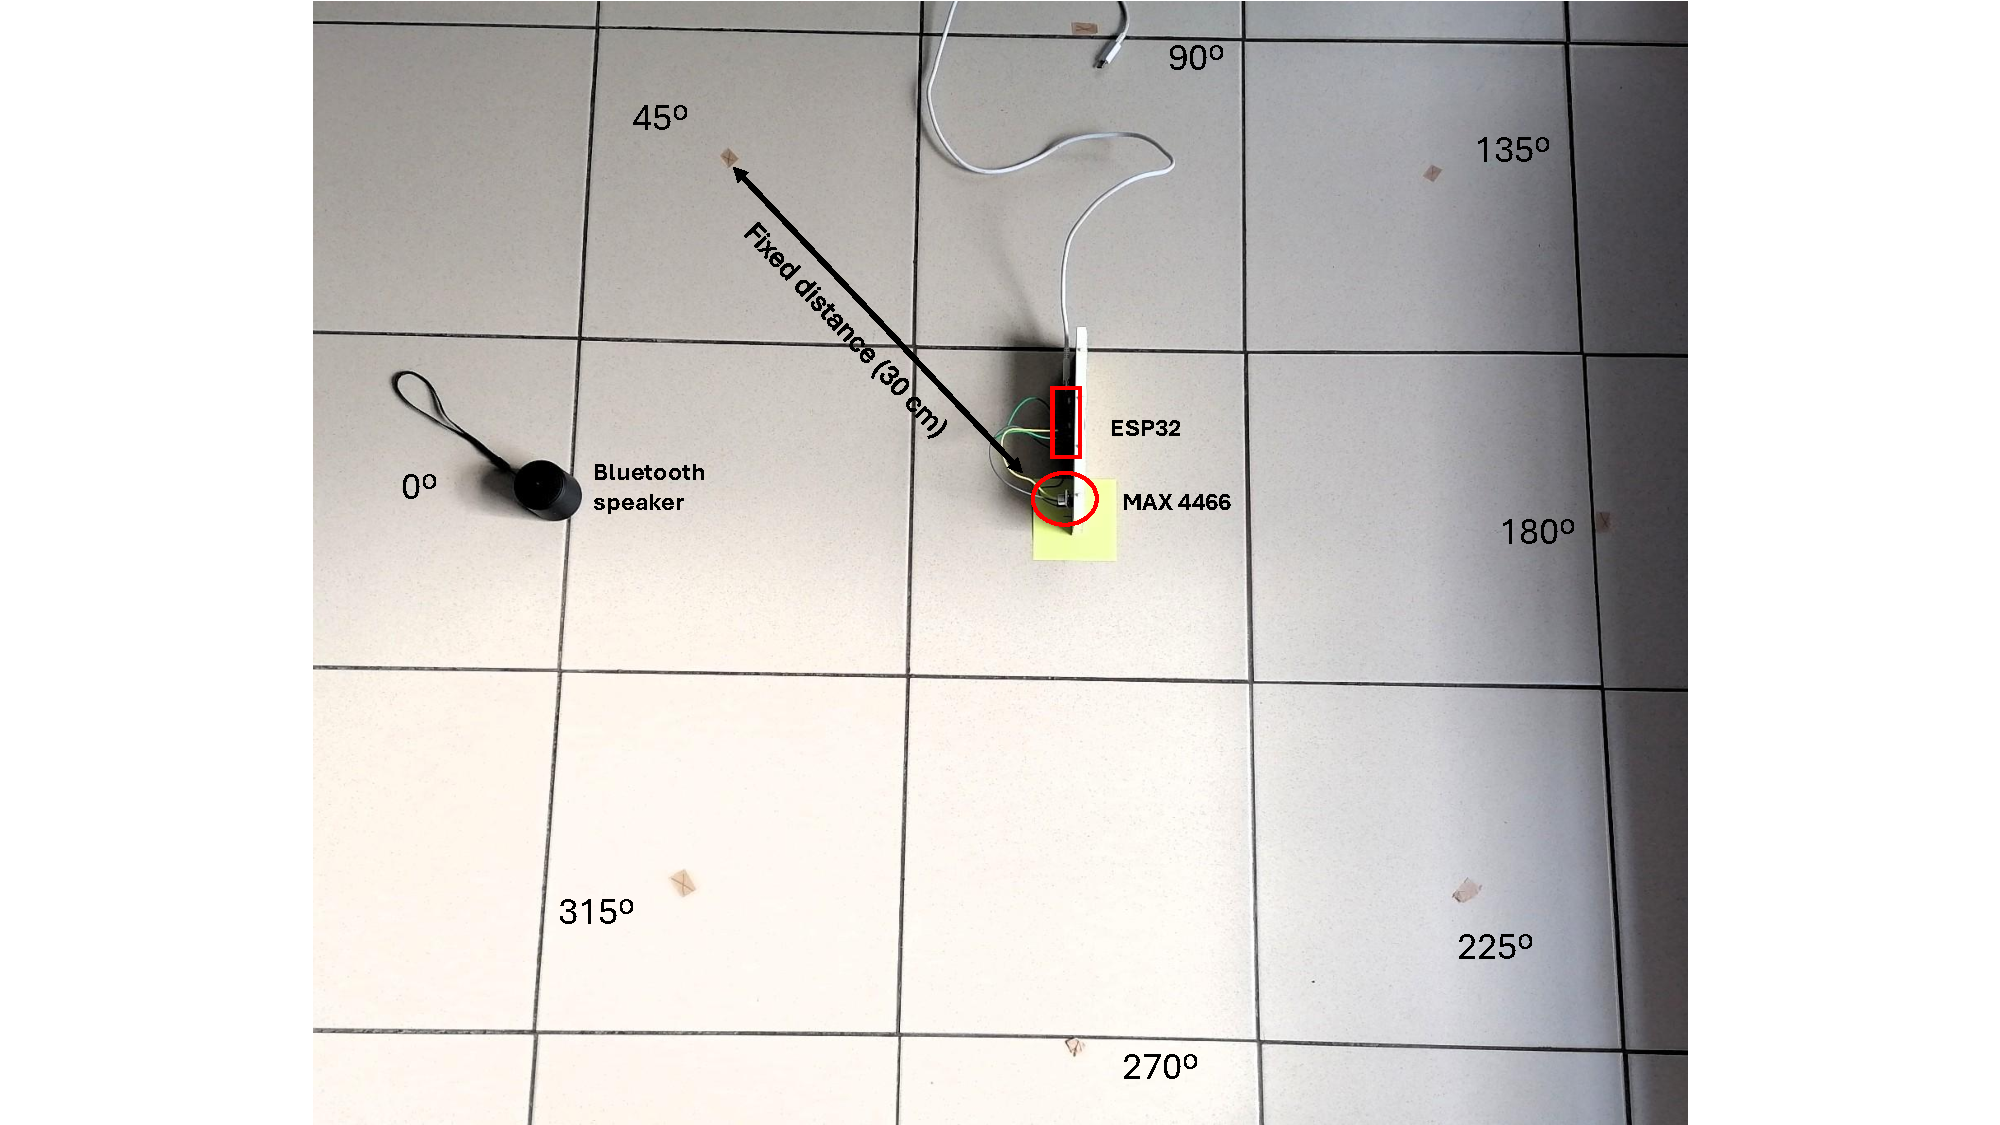
\includegraphics[width=0.7\linewidth]{poc.pdf}
    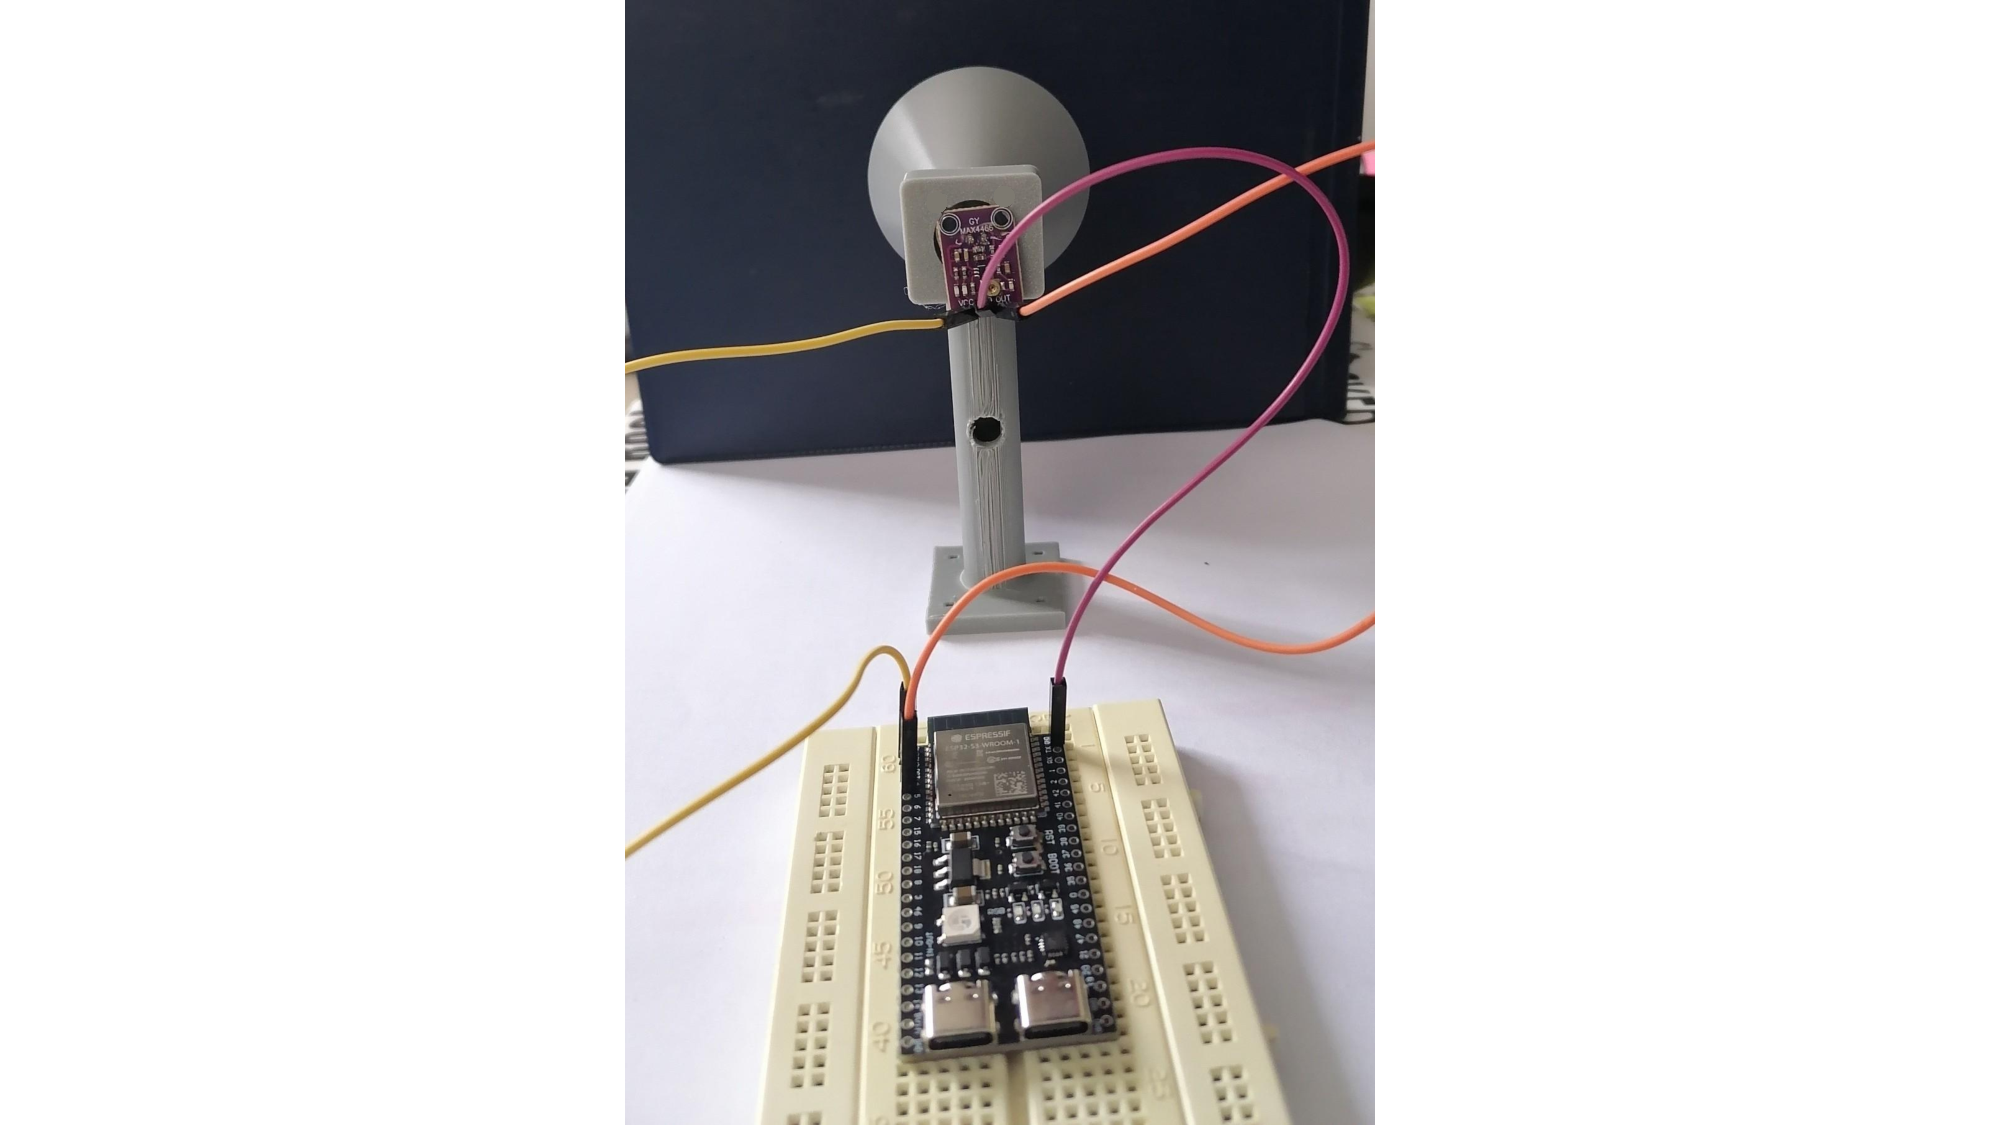
\includegraphics[width=0.2\linewidth]{mic_horn.pdf}
    \caption{Setup of the proof of concept including MAX 4466, ESP32, a breadboard, and a speaker with no horn (left) and zoom-in on the microphone + horn mounting for the second stage of the proof of concept (right).}
    \label{fig:poc}
\end{center}
\end{figure}

In the first stage, the microphone was connected to an ESP32 on a breadboard and placed at a fixed point, while a Bluetooth speaker was alternating across $8$ angular positions at a fixed distance of $30\text{ cm}$ (\autoref{fig:poc} left). The sound emitted consisted of a ``chirp'' at a constant frequency and regular intervals. Each angle sweep, at repeated measurements, exhibited peak-to-trough differences of approximately $5.2\text{--}7.8\text{ dB}$. The minimum amplitude was consistently recorded at $180^\circ$, while the maximum occurred near $0^\circ$ at around $63.0\text{ dB}$. Between $0^\circ$ and $180^\circ$, a drop of about $2\text{ dB}$ per $45^\circ$ was observed, with a symmetric behavior between $180^\circ$ and $360^\circ$ (\autoref{fig:polarplot} left). These results indicate the dependence of the response amplitude on the orientation of the sound source.

In the second stage, the same experiment was repeated with the 3D-printed directional horn attached to the microphone (\autoref{fig:poc} right). All other testing conditions were exactly the same. The results showed similar findings to the first stage of POC, but the signal level was approximately $2\text{ dB}$ higher in the horn pointing direction between $0^\circ\text{--}45^\circ$ and $315^\circ\text{--}360^\circ$, reaching approximately $65.0\text{ dB}$. This corresponds to a peak-to-trough difference of $10.3\text{--}10.5\text{ dB}$ (\autoref{fig:polarplot} right). This difference is higher than that recorded in the first stage, suggesting that the horn increases contrast of the measured signal between orientations. Therefore, these findings support the potential use of the horn in the assembly, although further testing at smaller angular increments is needed to achieve better sensitivity.

\begin{figure}[ht!]
\begin{center}
    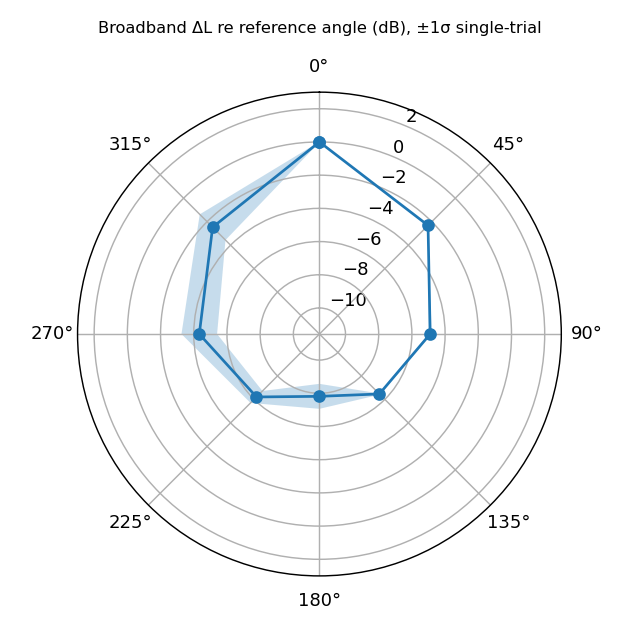
\includegraphics[width=0.43\linewidth]{bare1_summary_angle.png}
    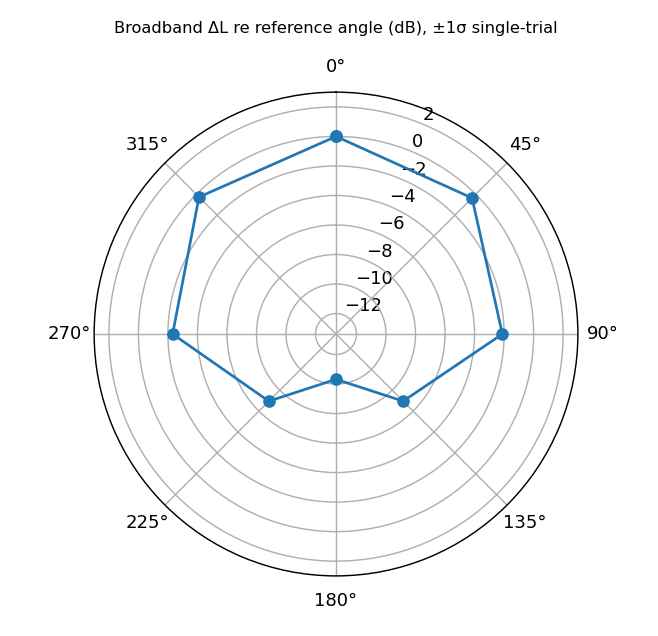
\includegraphics[width=0.43\linewidth]{horn1_summary_angle.png}
    \caption{\textbf{Measured directional gain profiles of the acoustic receiver setup.} Broadband relative sound level $\Delta L$ (dB) with respect to reference angle ($0^\circ$), evaluated across 8 angular increments ($45^\circ$ steps). \textbf{Left:} Baseline microphone setup without the directional horn. \textbf{Right:} Comparative profile with the 3D-printed directional horn.}
    \label{fig:polarplot}
\end{center}
\end{figure}


\textbf{Scope of the retained preliminary evidence.} This appendix reproduces the progress-report account. Its plotted levels are relative acquisition quantities, not calibrated acoustic sound-pressure levels. The original text uses ``chirp'' and ``constant frequency'' together; the waveform specification must be recovered from the acquisition record before drawing a frequency-specific conclusion. The coarse 30 cm experiment does not calibrate the operating-tone Gaussian model or establish metre-scale ranging accuracy.
\pending{P1 --- Preliminary-record reconciliation}{Verify the exact test waveform, level reference and raw-record links for the retained POC figures. Preserve the historical observations while distinguishing them from the new operating-tone calibration.}

\end{document}
